


\chapter{运动监测相关原理}
运动监测技术就是通过视觉或者传感器的数据,来估计用户的运动情况。在前文中,我们已经介绍HAR可以分为两类:基于视觉的HAR和基于穿戴式传感器的HAR。
基于视觉的HAR有许多局限性,例如摄像头等可视化工具通常是被固定的,更适合在室内使用,对于贯穿室内外以及不同地点的行为存在诸多限制,同时受光照、拍摄角度以及环境噪声的影响,难以提高分类精度。
与基于视觉的HAR相比,基于传感器的可穿戴HAR不受上述噪声的影响,可以实现更高的精度。
本章主要介绍基于穿戴式IMU的运动监测原理。


\section{人类活动识别原理}
\subsection{人类活动分类概述}



\subsection{常用算法}
\subsubsection{卷积神经网络}

\section{跌倒检测原理}
\subsection{跌倒过程}


\subsection{跌倒检测评估方法}
\subsection{常用算法}
\subsubsection{支持向量机算法}




\section{数据集}

\section{本章小结}




% \section{传感器及其应用简介}
% 论文主要涉及到三种传感器:加速度计、陀螺仪和气压计。为满足研究中传感器的要求,本文中所使用的IMU为维特智能公司生产的型号为HWT901B的集成传感器模块,包含三轴加速度计、三轴陀螺仪、三轴磁力计和气压计,
% 如图\ref{imu}所示。本文中使用的都是微机电系统(Micro­Electro Mechanical Systems,MEMS)下的传感器,由于构成原理和制作工艺等方面的因素,MEMS 传感器具有更多良好的特性,如成本低、可靠性高、功耗低和体积小等等优点。在介绍具体算法之前,本节先对这三种传感进行简单介绍。

% 	\begin{figure}[h]
% 		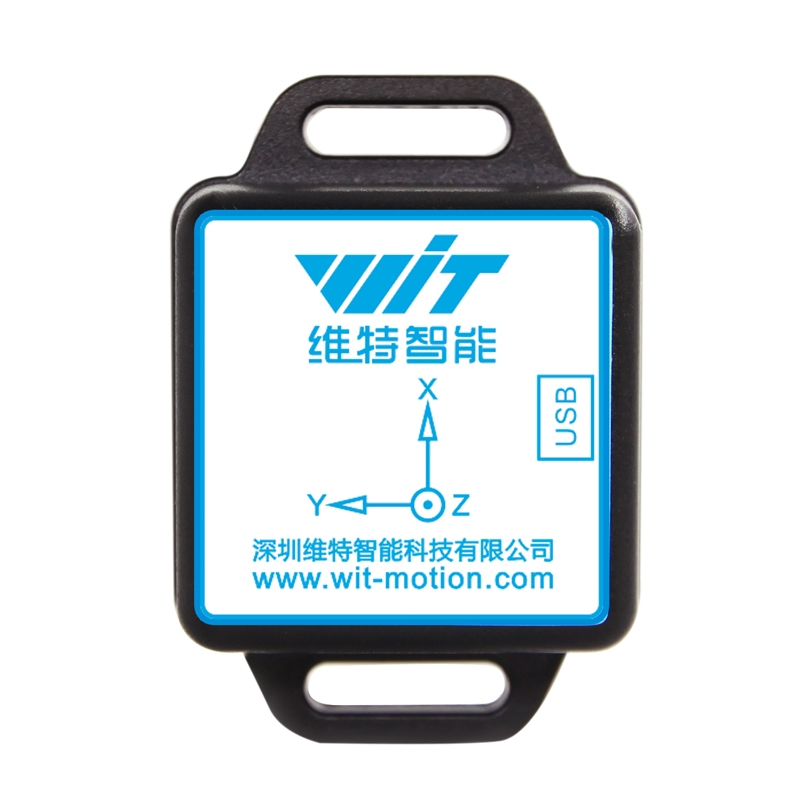
\includegraphics[width=0.3\textwidth]{IMU.jpg}
% 		\caption{RWG 基函数几何参数示意图}
% 		\label{imu}
% 	\end{figure}


% \subsection{加速度计}
% % 可以借用  基于改进CNN-LSTM的人体行为识别研究_龙秋玲  中2.1.1

% 加速度计是一种惯性传感器,它能够测量物体的加速度。当加速度计与物体一起运动时,能够将加速度转化为输出信号。目前常用的是MEMS加速度计,由于采用了微机电系统技术,使得其尺寸大大缩小,一个MEMS加速度计只有指甲盖的几分之一大小。MEMS加速度计具有体积小、重量轻、能耗低等优点。

% 本文所用到是三轴加速度计,三个轴的方向互相垂直构成一个空间直角坐标系,即加速度计的输出分别是载体在空间相互垂直的三个方向上的数据。因此,当加速度计静置于水平地面上时,由于加速度计本身与地面相对静止,加速度计三轴的一个必定与地面垂直,如图\ref{acc}所示。此时加速度计仅受到地心引力的作用,因此其三轴输出中,仅有跟地面垂直的那个轴有读数,而且读数的绝对值应该是在重力加速度 g 附近小幅度波动,而另外两个轴的读数应该是在 0 附近小幅度波动,这种波动产生则是由传感器本身以及周围的环境噪声引起的。

% \begin{figure}[h]
% 	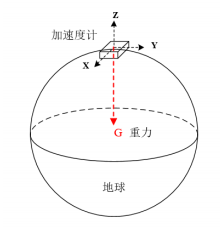
\includegraphics[width=0.3\textwidth]{acc.jpg}
% 	\caption{RWG 加速度计静置与水平地面示意图}
% 	\label{acc}
% \end{figure}

% % 由于重力加速度的存在,静置于水平地面的加速度计的垂直于水平面的轴的读数正好是重力加速度g,利用这种特性,当加速度计至于非水平地面上时,重力的方向将不再与原轴重合,而是可以将其以某个角度分解至两个轴上,如图 2­2 所示。因此可以通过加速度计三轴的读数,结合三角函数即可得到加速度计当前所处位置与水平面所成的角度关系。 田园师兄论文出处

% 将加速度计放在人身上,人体在日常生活中会不断做出各种动作,加速度会伴随动作一起出现,利用加速度计采集这些加速度信息就可以得到人体运动的加速度信息,通过科学的方法进行处理和分析,就可以用来监测人们的日常行为,从而更好的改善人们的生活。


% \subsection{陀螺仪}

% 可能涉及不到,暂定!

% \subsection{气压计}
% % 可以借用 基于智能手机多传感器融合技术的人体活动识别研究_杨佳现   中2.2.2  章内容
% 气压传感器主要用于测量大气压强,气压国际制单位是帕斯卡,简称帕,符号是Pa。其中MEMS气压传感器主要原理是压电效应,压电材料可以产生电流。当它们受到外力的作用时,材料会产生形变,其内部会产生极化现象,在形变的两端出现正负等量的电荷。首先,电流可以用来计算材料的形变程度,然后材料的形变可以用来计算外力大小,因此探测电流就可以计算出外力大小。

% 这类MEMS压力传感器本质上是一个空气腔,其一侧带有类似气球的柔性材料。当传感器位于气压较高的区域(例如低谷)时,膜就会由于外界压力变大而被推向腔内。当传感器位于气压低的区域(例如山峰),膜会从腔体中凸出。在这层膜上附有敏感材料。传感器可以读取材料(形变)产生的电流变化,然后通过该电流读数计算出施加到膜上的压力。接下来,因为腔内的压力已知,那么传感器就可以计算出外部压力大小。

% 气压传感器用途广泛,用户通过气压传感器可计算得出测量设备所处的海拔高度,进而提高利用智能手机进行定位的可靠性和精准度,也可直接用来进行辅助设备的 GPS 定位,来帮助用户确认设备所在楼层的位置等相关信息。


% \section{基于IMU的运动监测技术}
% 基于IMU的运动监测技术的整个工作原理如下:首先从多个传感器收集数据,如加速度计、陀螺仪和气压计,这些传感器放置在大腿、腰部等,然后对数据进行滤波等处理,最后进行特征提取和分类。
% 在本文中,基于IMU的运动监测技术主要包含三个方面:人类活动识别、步行稳定性和跌倒检测。

% \subsection{人类活动识别}
% % 主要介绍目前有哪些方法可以进行识别,各有什么优点
% 人类活动识别主要是采集人类活动时的各种数据,通过某种方法,正确的分析出人类当前的运动状态,本文主要研究站立,走路,上楼,下楼这四个运动状态。在上一小节中,我们已经介绍了加速度计可以反映人体运动的加速度信息,所以可以根据加速度信息来对人类活动进行识别。

% 人类活动识别目前通用流程如图\ref{har1}所示,首先佩戴加速度传感器采集大量的活动数据,然后原始数据进行一系列的处理,由于数据中包含了各种各样的噪声,因此需要对原始数据进行预处理,例如分割和滤波等。预处理后的加速度数据经过特征选取组成特征矩阵,然后送入分类器进行模型训练和识别分类工作。训练好的模型将被用于识别过程中,在识别分类的时候,分类器需要用到待识别样本的特征矢量和之前训练好的分类模型,分类器会在两者么间进行匹配计算,使用特定的匹配算法,进而计算出两者之间的相似度,选出相似度最高的模板,将待识别样本归入到此类中,即得到了识别分类的结果。


% \begin{figure}[h]
% 	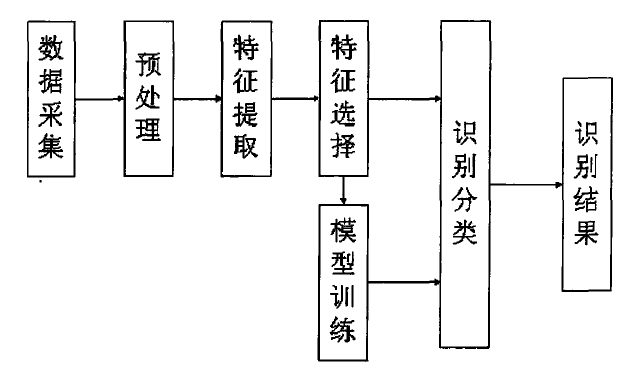
\includegraphics[width=0.5\textwidth]{har1.jpg}
% 	\caption{RWG 基于3轴加速度传感器的人体行为识别常用识别过程}
% 	\label{har1}
% \end{figure}

% \subsection{步行稳定性}
% \subsection{跌倒检测}

% % 参考论文   A Combined Smartphone and Smartwatch Fall Detection System

% 跌倒前阶段:受试者从事的日常生活的初始活动

% 自由落体阶段:由于失去平衡而向地面自由落体运动

% 撞击阶段:代表物体接触表面的那一刻的撞击

% 撞击后阶段:撞击后的瞬间,当人因跌落的冲击而躺在地板上时

% 恢复阶段:受试者努力站起来或从跌倒中恢复


% \section{本章小结}



% \subsection{空间基函数}
% RWG 基函数是定义在三角形单元上的最具代表性的基函数。它的具体定义如下:
% \begin{equation}
% f_n(\bm{r})=
% \begin{cases}
% \frac{l_n}{2A_n^+}\bm{\rho}_n^+=\frac{l_n}{2A_n^+}(\bm{r}-\bm{r}_+)&\bm{r}\in T_n^+\\
% \frac{l_n}{2A_n^-}\bm{\rho}_n^-=\frac{l_n}{2A_n^-}(\bm{r}_--\bm{r})&\bm{r}\in T_n^-\\
% 0&\text{otherwise}
% \end{cases}
% \end{equation}

% 其中,$l_n$为三角形单元$T_n^+$和$T_n^-$公共边的长度,$A_n^+$和$A_n^-$分别为三角形单元$T_n^+$和$T_n^-$的面积(如图\ref{pica}所示)。

% \begin{figure}[h]
% 	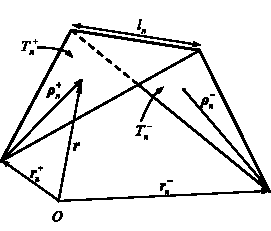
\includegraphics{pica.pdf}
% 	\caption{RWG 基函数几何参数示意图}
% 	\label{pica}
% \end{figure}

% 由于时域混合场积分方程是时域电场积分方程与时域磁场积分方程的线性组合,因此时域混合场积分方程时间步进算法的阻抗矩阵特征与时域电场积分方程时间步进算法的阻抗矩阵特征相同。
% \begin{equation}
% \label{latent_binary_variable}
% \bm{r}_{i,j}=
% \begin{cases}
% 1,f(\bm{x}^{i};\bm{w})\cdot f(\bm{x}^{j};\bm{w})\geq u(\lambda),\\
% 0,f(\bm{x}^{i};\bm{w})\cdot f(\bm{x}^{j};\bm{w})< l(\lambda), 1\leq i,j\leq n.\\
% f(\bm{x}^{i};\bm{w})\cdot f(\bm{x}^{j};\bm{w}),\text{otherwise},
% \end{cases}
% \end{equation}

% 时域积分方程时间步进算法的阻抗元素直接影响算法的后时稳定性,因此阻抗元素的计算是算法的关键之一,采用精度高效的方法计算时域阻抗元素是时域积分方程时间步进算法研究的重点之一。


% \subsection{时间基函数}

% \subsubsection{时域方法特有的展开函数}

% \subsubsection{频域方法特有的展开函数}

% \section{入射波}

% 如图\ref{picb}和图\ref{picc}所示分别给出了参数$E_0=\hat{x}$,$a_n=-\hat{z}$,$f_0=250MHz$,$f_w=50MHz$,$t_w=4.2\sigma$时,调制高斯脉冲的时域与频域归一化波形图。

% \begin{figure}[h]
% \subfloat[]{
% 	\label{picb}
% 	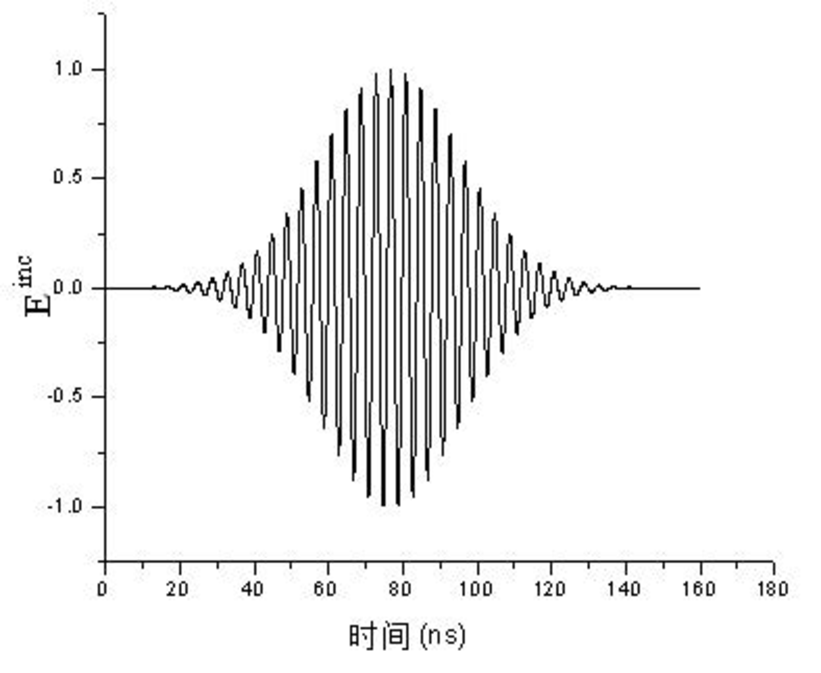
\includegraphics[width=7.3cm]{picb.pdf}
% }
% \subfloat[]{
% 	\label{picc}
% 	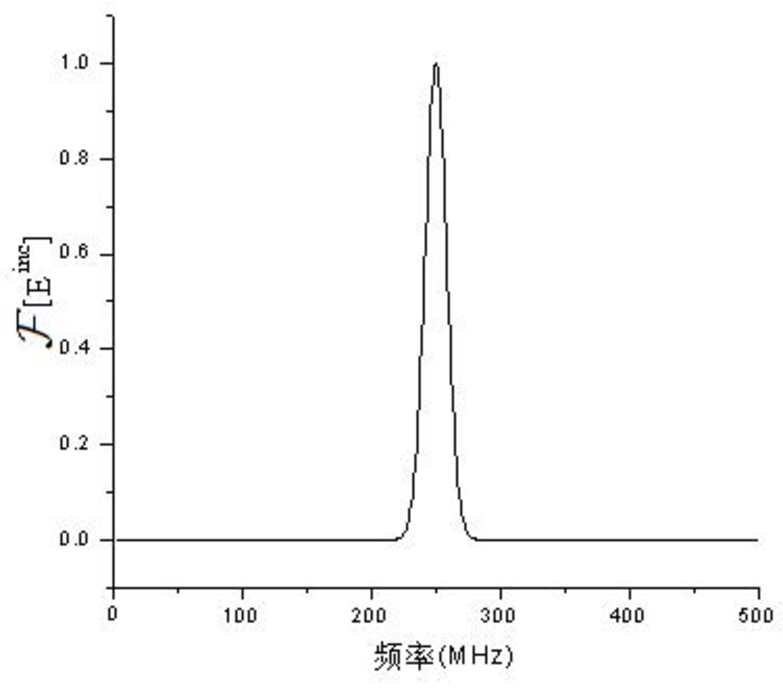
\includegraphics[width=6.41cm]{picc.pdf}
% }
% \caption{调制高斯脉冲时域与频率波形,时域阻抗元素的存储技术也是时间步进算法并行化的关键技术之一。(a)调制高斯脉冲信号的时域波形;(b)调制高斯脉冲信号的频域波形}
% \label{fig1}
% \end{figure}

% 时域阻抗元素的存储技术\citing{xiao2012yi}也是时间步进算法并行化的关键技术之一,采用合适的阻抗元素存储方式可以很大的提高并行时间步进算法的计算效率。

% \section{本章小结}
% 本章首先从时域麦克斯韦方程组出发推导得到了时域电场、磁场以及混合场积分方程。
